
% Author: Charlie Albright, Spencer Kaiser, Luke Oglesbee
% Creation Date: 9 October 2014
% Version: 1.0
%
\documentclass{sigcomm-alternate}
\usepackage{cite}
\usepackage{fancybox}
\usepackage{pseudocode}
\usepackage{pgfplots}

\title{
Error Correction Coding in Passive UHF Gen2 Communications\\
{\large CSE 4344}
}

\numberofauthors{3}
\author{
\alignauthor Charlie A. Albright\\
\affaddr{Computer Science and Engineering Department\\
 	Southern Methodist University\\
	Dallas, Texas USA}\\
\email{calbright@smu.edu}
%
\alignauthor Spencer A. Kaiser\\
\affaddr{Computer Science and Engineering Department\\
 	Southern Methodist University\\
	Dallas, Texas USA}\\
\email{skaiser@smu.edu}
%
\alignauthor Luke W. Oglesbee\\
\affaddr{Computer Science and Engineering Department\\
 	Southern Methodist University\\
	Dallas, Texas USA}\\
\email{loglesbee@smu.edu}
}

\begin{document}


\maketitle

\section{graph}
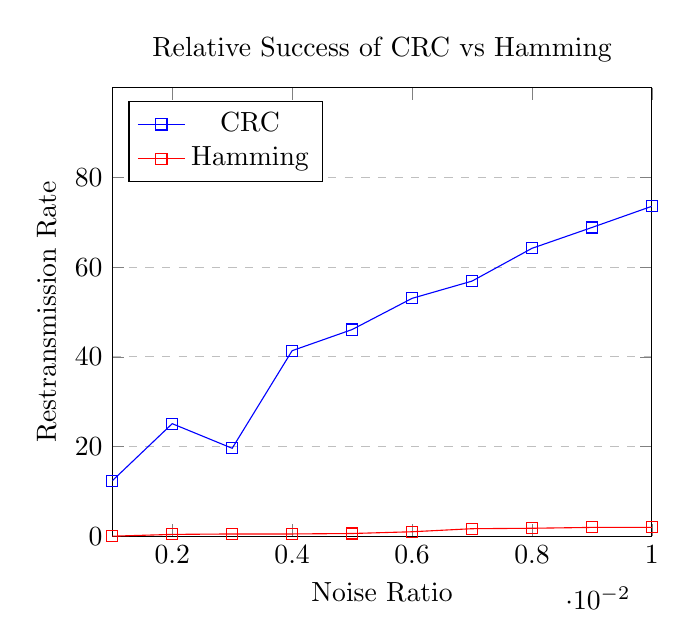
\begin{tikzpicture}
\begin{axis}[
    title={Relative Success of CRC vs Hamming},
    xlabel={Noise Ratio},
    ylabel={Restransmission Rate},
    xmin=0.001, xmax=0.01,
    ymin=0, ymax=100,
    xtick={0.002,0.004,0.006,0.008,0.01}, %,0.012,0.014,0.016,0.018},
    ytick={0,20,40,60,80},
    legend pos=north west,
    ymajorgrids=true,
    grid style=dashed,
]
\addplot[
    color=blue,
    mark=square,
    ]
    coordinates {
    (0.001,12.36)(0.002,25.1)(0.003,19.61)(0.004,41.38)(0.005,46.09)
    (0.006,53.05)(0.007,56.9)(0.008,64.21)(0.009,68.86)(0.01,73.59)
    };
\addplot[
    color=red,
    mark=square,
    ]
    coordinates {
    (0.001,0)(0.002,0.4)(0.003,0.5)(0.004,0.5)(0.005,0.6)
    (0.006,0.99)(0.007,1.67)(0.008,1.77)(0.009,1.96)(0.01,1.96)
    };
    \legend{CRC, Hamming}
 
\end{axis}
\end{tikzpicture}

% \section{Introduction}
% The purpose of this study is to explore possible error-correcting alternatives to the simple Cyclic Redundancy Check (CRC) codes used in Ultra-High Frequency (UHF) Gen2 RFID communications. We will evaluate the complexity added to the RFID system when using various types of error-correcting codes and analyze their effects on the performance of the system. We will also compute the additional circuitry needed to implement our alternatives to CRC, and then weigh the benefits and cost of implementing this particular Error-Correcting Code (ECC) into RFID communications.

% As of current, RFID uses Cyclic Redundancy Checks (CRC) to detect errors that happen when the information is transmitted wirelessly from Tag to Reader and from Reader to Tag. However, even if these errors are detected, the system is not able to correct the error, so the result is thrown out and another request for the Tag's ID is made. We propose that if the RFID system was able to correct one-bit or even multiple-bit errors, RFID's reliability and overall success would benefit significantly. By having an error-correcting system implemented, the Reader would be able to identify the Tag in less reads on average, and it would potentially improve the range at which the Reader could identify the Tag.

% \section{Methodology}
% \textbf{SHOULD WE KEEP SOME OR ALL OF THIS?}

% The first major milestone in approaching our research problem will be to develop a firm understanding of the implementation and execution of Cyclic Redundancy Check (CRC) in the context of RFID interrogators. This will be accomplished through an analysis of the Class-1 Generation-2 UHF RFID documentation provided by EPCglobal and by examining past work in the RFID communications field, specifically with regards to the use of CRC.
	
% After establishing a thorough understanding of CRC, our next step will be to delve into the execution of error-correcting code. We will do this by reviewing past work that identifies the key differentiations and variations in performance between the two codes. We will then identify one or more specific error-correcting codes that we believe to be most applicable for use in RFID systems and conduct further research regarding these specific codes. 

% Finally, once we have developed a deep understanding of CRC and identified one or more error-correcting codes for use in an RFID system, we will transmission error rate metrics for RFID systems to simulate the effect of these error correcting codes in terms of tag reading efficiency, added complexity to the tag and interrogator, and overall performance increase for the system.

% \section{Previous Work}
% In their article, A New Ultralightweight RFID Authentication Protocol with Permutation, authors Tian, Chen, and Li propose implementing a strong but relatively simple protocol that implements permutation in order to establish authenticity between Reader and Tag\cite{3}. The last messages exchanged in their protocol are sent again by the reader to resist against desynchronization attacks.

% Authors Grzegorz Smietanka, Jan Geldmacher and Jurgen Gotze proposed the implementation of Forward Error Correction (FEC) in their article, Error Detection Based on Correlation Analysis for BCH Encoded UHF RFID Communication\cite{1}. They say the FEC could be implemented easily because of BCH code?s similarity to CRC. 

% A Secure RFID Authentication Protocol Adopting Error Correction Code talks about using a one-way hash to establish authenticity and prevent intentional transmission manipulation, which CRC is not capable of detecting. By hashing the Tag's ID, a secret key, and random challenge numbers, the authors claim that mutual authentication can be achieved\cite{5}.

% Another lightweight protocol for de-synchronization is proposed by authors Zhou, Zhang, Luo, and Wong in their article A lightweight anti-desynchronization RFID authentication protocol. They claim that using the one-way hash and XOR functions while the backend server keeps a history of all shared secret keys prevents desynchronization and is capable of finding intentional errors \cite{4}.

% Finally, On Error Performance Improvements of Passive UHF RFID Systems via Syndrome Decoding discusses using the existing CRC error detection implementation to correct single bit errors. Using a lookup table with various CRC codes and other information stored in it, CRC becomes capable of correcting single bit errors\cite{2}.

% \section{Implementation and Testing}
% In order to test the effects of adding an error-correcting code in place of the CRC that is already in place for RFID communications, we decided to implement a virtual testing environment comprised of completely software. We put considerable time and thought into carefully choosing which language to implement our environment in, and after weighing the pros and cons, we chose to write our testing modules in Python. We felt that Python's unique functionality, ingenious string manipulation methods, and overall lightweight qualities would be well suited for rapid processing of simulated transmissions.

% The general setup of our testing environment runs in a main file, with specific Python modules included for each Noise model and ECC implementation, which are written in separate files. Our main file simulates an RFID reader unit by opening a text file containing a sample packet on each line. The testing environment then runs each packet through a series of Error-Correcting Codes and Noise models and analyzes the results of the fake transmission, keeping track of variable such as the total number of transmissions, the number of times a retransmission occurred, and how often the ECC was able to correct the errors. the Following algorithm gives an overview of the overall process that a packet goes through:

% \begin{pseudocode}{Packet Analysis}{Parameters}
% \FOREACH Packet \in File 
% 	\DO
% 	\BEGIN
% 		Encode\ Packet\ with\ CRC\\
% 		\WHILE Transmission\ is\ not\ successful
% 			\DO
% 			\BEGIN
% 				Send\ Packet\ though\ Noise\ module\\
% 				Decode\ resulting\ Packet\ to\ check\ for\ errors\\
% 				\IF Errors\ Detected
% 					\THEN
% 					\BEGIN
% 						Retransmission\ occurs
% 					\END
% 				\ELSEIF Errors\ exist\ but\ undetected
% 					\THEN
% 					\BEGIN
% 						Undetected\ Error\ occurs
% 					\END
% 				\ELSE
% 					Successful\ transmission
% 			\END\\\\
% 		Encode\ Packet\ With\ Hamming\\
% 		\WHILE Transmission\ is\ not\ successful
% 			\DO
% 			\BEGIN
% 				Send\ Packet\ though\ Noise\ module\\
% 				Decode\ resulting\ Packet\ to\ check\ for\ errors\\
% 				\IF Errors\ Detected\ and\ Not\ Fixed
% 					\THEN
% 					\BEGIN
% 						Retransmission\ occurs
% 					\END
% 				\ELSEIF Errors\ exist\ but\ undetected
% 					\THEN
% 					\BEGIN
% 						Undetected\ Error\ occurs
% 					\END
% 				\ELSE
% 					Successful\ transmission
% 			\END
% 	\END\\\\
	
% Print\ results\ to\ screen
% \end{pseudocode}

% \begin{pseudocode}{Hamming}{Signal}
% 	\PROCEDURE{Encode}{Signal}
% 		% Output \GETS [0]\\
% 		% ParityBits \GETS [1]\\
% 		% i \GETS 2\\
% 		\mbox{Insert empty parity bits into } Signal\\
% 		% \WHILE i < length(Signal) \DO
% 		% 	\BEGIN
% 		% 		\IF i \mbox{ is power of two}
% 		% 		\THEN
% 		% 			\BEGIN
% 		% 				ParityBits \mbox{ push } i\\
% 		% 				Output \mbox{ push } Signal[i]\\
% 		% 				i \GETS i+1\\
% 		% 			\END\\
% 		% 		\BEGIN
% 		% 			Output \mbox{ push } Signal[i]\\
% 		% 			i \GETS i+1
% 		% 		\END
% 		% 	\END\\
% 		\FOREACH parityBit \mbox{ in } Signal \DO
% 			% \BEGIN
% 				Signal[parityBit-1] \GETS Parity(Signal, parityBit)\\
% 			% \END\\
% 		\RETURN{Signal}
% 	\ENDPROCEDURE

% 	\PROCEDURE{Decode}{Signal}
% 		\FOREACH parityBit \mbox{ in } Signal \DO
% 			\BEGIN
% 				\IF Parity(Signal, parityBit) == 1
% 				\THEN
% 					ParityErrors \mbox{ push } parityBit
% 			\END\\
% 		\IF ParityErrors
% 		\THEN
% 			\BEGIN
% 				badBit \GETS \mbox{sum of } ParityErrrors\\
% 				\IF badBit \geq length(Signal)
% 				\THEN
% 					\RETURN{False}
% 				\ELSE
% 					Signal[badBit-1] \GETS !Signal[badBit-1]
% 			\END\\
% 		\mbox{Remove parity bits from } Signal\\
% 		\RETURN{Signal}
% 	\ENDPROCEDURE

% 	\PROCEDURE{Parity}{Signal, parityBit}
% 		i \GETS parityBits\\
% 		comp \GETS Signal[parityBits-1]\\
% 		\WHILE i < length(Signal) \DO
% 			\BEGIN
% 				j \GETS i\\
% 				\WHILE j < i+parityBit \AND j < length(Signal) \DO
% 					\BEGIN
% 						comp = comp \oplus Signal[j]\\
% 						j \GETS j+1
% 					\END\\
% 				i \GETS i + 2 \cdot parityBit
% 			\END\\
% 	\RETURN{comp}
% 	\ENDPROCEDURE
% \end{pseudocode}

% \begin{pseudocode}{Gaussian Noise}{Signal, noiseRatio}
% 	Noise \GETS \mbox{random value (0-1) for each element of } Signal\\
% 	\FOR i \GETS 0 \TO length(Signal) \DO
% 		\BEGIN
% 			\IF Signal[i] < noiseRatio
% 			\THEN
% 				Signal[i] \GETS !Signal[i]
% 			\ELSE
% 				Signal[i] \GETS Signal[i]
% 		\END\\
% 	\RETURN{Signal}
% \end{pseudocode}

% \begin{pseudocode}{Burst Noise}{Signal, noiseRatio, maxBitFlip=16}
% 	Noise \GETS \mbox{random float (0-1) for each element of } Signal\\
% 	Length \GETS \mbox{random int (0-maxBitFlip) for each element of } Signal\\
% 	i \GETS 0\\	
% 	\WHILE i < length(Signal) \DO
% 		\BEGIN
% 			\IF Signal[i] < noiseRatio
% 			\THEN
% 				\BEGIN
% 					\FOR j \GETS i \TO i+Length[i] \DO
% 						\BEGIN
% 							Signal[j] \GETS !Signal[j]
% 						\END\\
% 					i \GETS i + j\\
% 				\END
% 			\ELSE
% 				i \GETS i + 1
% 		\END\\
% 	\RETURN{Signal}
% \end{pseudocode}

% \section{Revised Research Plan}

% \textbf{11/11/14: Interim report}

% 11/12 - 11/16: Implement missing Noise and ECC models

% 11/17 - 11/21: Perform final analysis on effectiveness on each Error Correcting Code for each Noise Model and collect data for comparison

% 11/22 - 11/27: FINAL WORK PERIOD - Make final additions to paper and revise

% 11/28: Assign presentation sub-sections to team members

% 11/28 - 12/1: Team members individually create presentation components

% 12/1 - TBD: Compile final presentation from components and practice delivery

% \textbf{TBD (12/2/14 - 12/4/14): Final Presentation}

% \section{Road Blocks and Concerns}
% The major road block we have is finding a quantitative method to measure the efficacy of a protocol in a theoretical environment. Most past work on efficacy of error-correcting protocols in RFID communication has been conducted in controlled laboratory environments. While a statistical analysis based on the chance of message bits being corrupted under various conditions is plausible, we have not yet found any pre-existing methods for conducting the analysis.

\nocite{*}
\bibliographystyle{plain}
\bibliography{AlbrightKaiserOglesbeeInterimReport} 

\balancecolumns
%---- End the Document
\end{document}




